\section{Hunter's Guild}
\label{sec:Hunters Guild}

\begin{figure}[!ht]
  \centering
  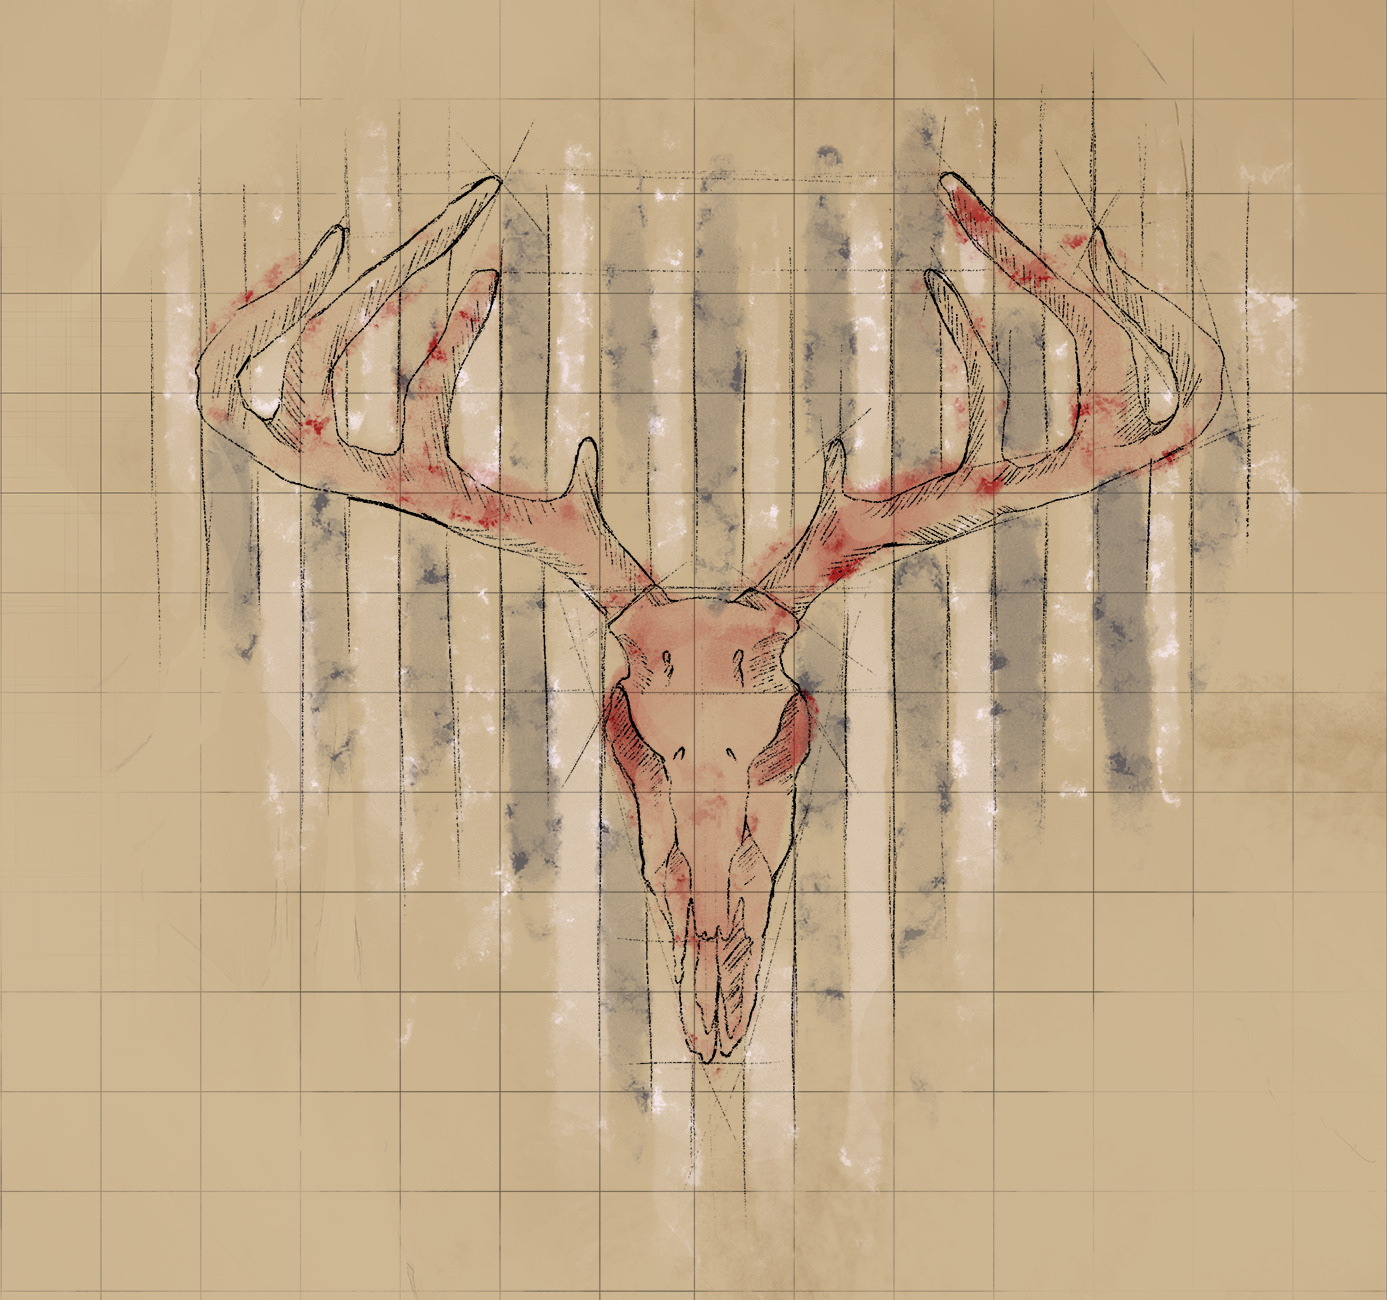
\includegraphics[width=0.9\linewidth]{media/norbury-huntersguildsm.png}
\end{figure}

The \emph{Hunter's Guild} is the slavery guild of \nameref{sec:Norbury}. It is
tasked with marking and handling new slaves, keeping track of existing ones,
and tracking down and returning those that have escaped. It operates an office
building and a large auction hall in the main square of the city.

The hunter's guild banner is a skull of a deer (with antlers) painted in red
upon a white background.

The guilds main income is the auction, and various administrative fees it
collects for transferring or freeing slaves. It does not charge for retrieving
runaway slaves, or for registering new slaves into the kingdom. The guild is
the main source of income for most soldiers of the Norbury army, as they pay a
share of the auction's profit for all soldiers who bring them new slaves to
sell. Many third party slavers or other slaving nations often trade goods with
the hunter's guild.

A lesser known duty of the Guild is to rescue Norbury citizens from slavery in
other slaving nations or city kingdoms. Although technically not bound by law
to do so, it often extends this service to any citizens of kingdoms that have
signed the \nameref{sec:Vonir Accord}. For these clandestine tasks it hires
special agents, spies and assassins whose rescue operations often bring them
in direct conflict with other slavers, such as the \nameref{sec:Velvet Hand}.

It also employs \emph{hunters}, often rangers, barbarians, fighters and
rogues, that are tasked with tracking down escaped slaves. These hunters are
also allowed to enslave people, although they rarely do so. The guild
has a troubled past with enslaving citizens of other city kingdoms and allied
nations, and has thus issued decrees for its hunters to go only after their
designated targets.

Although hunters make up a lion share of people employed by the guild, it also
hires bureaucrats, taskmasters and wizards. These wizards are responsible for
developing the \nameref{sec:Slave Band} as the \hyperref[sec:Slave Mark]{slave
  runes}, arcane contraptions to bind and track slaves. The bureaucrats are
mostly responsible for tracking, organising, and categorising slaves, as well
as organising auctions and large scale trades. They are also responsible for
developing the colour code and classification system for slaves: \emph{White}
means that the slave is ``valueless'' or ``useless''. \emph{Gray} coloured
slaves have no special qualities or skills. \emph{Green} slaves have a special
skill that makes them valuable, which is often inscribed with a symbol right
next to the green identification mark. \emph{Red} slaves have no current
owner, and \emph{black} denotes slaves of high value. These are often
specialised craftsmen, priced fighters or perhaps slaves with magical
talents. Any of these colours may be combined with each other to easily signal
the current status of the slave.

The guilds mostly operates within the borders of the city kingdom, as well as
the outlying baronies and smaller kingdoms and any nation or city kingdom
that signed the \nameref{sec:Vonir Accord}. The guild is banned from operating
in city kingdoms and baronies that have banned slavery, but still does so, often
in secret.

\begin{35e}{Hunter's Guild}
  The Hunter's Guild is considered \emph{lawful evil}, and will hire anyone that
  has proven himself reliable, mindful of the respective laws (such as the Vonir
  Accord), and a skilled.
\end{35e}
